

\chapter{Opis struktury projektu}
\label{chap:struktura_projektu}
W niniejszym rozdziale przedstawiono zaprojektowaną strukturę projektu wraz z jej opisem technicznym. Opisane zostały także wykorzystane technologie, zarządzanie danymi oraz baza danych. Uwzględniono również informacje dotyczące hierarchii klas, najważniejszych metod oraz wymagań systemowych.

\section{Wykorzystane technologie i narzędzia}
Do realizacji projektu wykorzystano szereg sprawdzonych technologii. Głównym językiem programowania jest \textbf{Java}, wybrana ze względu na jej obiektowość, przenośność i bogatą bibliotekę standardową. Interfejs graficzny użytkownika (GUI) został zaimplementowany przy użyciu biblioteki \textbf{Java Swing}, która umożliwiła stworzenie interaktywnego interfejsu desktopowego. Za przechowywanie danych odpowiada system zarządzania bazą danych \textbf{MySQL}, a komunikacja między aplikacją a bazą danych odbywa się za pośrednictwem sterownika \textbf{JDBC}. Kod źródłowy projektu był zarządzany przez system kontroli wersji \textbf{Git} przy użyciu klienta zintegrowanego ze środowiskiem \textbf{IntelliJ IDEA}, a centralne repozytorium zostało umieszczone na platformie \textbf{GitHub}. W celu poprawy użyteczności interfejsu, zintegrowano zewnętrzną bibliotekę \textbf{LGoodDatePicker} \cite{LGoodDatePicker}.

\section{Architektura i hierarchia klas}
Aplikacja została zaprojektowana w oparciu o architekturę trójwarstwową, która separuje od siebie poszczególne części systemu, zwiększając jego modularność i ułatwiając rozwój.

\begin{enumerate}
    \item \textbf{Warstwa Prezentacji (View):} Jest to warstwa interfejsu graficznego, zaimplementowana w pakiecie `View` przy użyciu biblioteki Java Swing. Obejmuje ona wszystkie klasy odpowiedzialne za wyświetlanie okien i interakcję z użytkownikiem, takie jak \texttt{MainForm.java}, \texttt{AdminForm.java}, \texttt{ShopRetailForm.java} oraz \texttt{ShopWholeSaleForm.java}.
    
    \item \textbf{Warstwa Logiki Biznesowej (Model):} Ta warstwa, zlokalizowana w pakiecie `Model`, zawiera logikę działania aplikacji oraz obiekty modelujące dane. Znajdują się tu klasy modelu, takie jak \texttt{Product.java} wraz z jej podklasami (np. \texttt{ProductClothes.java}, \texttt{ProductElectric.java}), \texttt{Cart.java} do zarządzania koszykiem, oraz \texttt{Customer.java} reprezentująca klienta. Do kluczowych metod w tej warstwie należą \texttt{Cart.dodajProdukt()}, pozwalająca na dodawanie produktów do koszyka, oraz \texttt{Cart.obliczCalkowitaSume()}, która dynamicznie oblicza jego wartość.
    
    \item \textbf{Warstwa Dostępu do Danych (Data Access Layer):} Warstwa ta odpowiada za całą komunikację z bazą danych i została zaimplementowana w pakiecie `DAO` z wykorzystaniem wzorca projektowego \textbf{Data Access Object}. Dzięki temu operacje na bazie danych (CRUD) są całkowicie odizolowane od reszty aplikacji. Główne komponenty tej warstwy to klasy DAO, takie jak \texttt{ProductsDAO.java}, \texttt{UserDAO.java} oraz \texttt{OrderDAO.java}. Niezwykle istotną metodą jest \texttt{DatabaseConnection.getConnection()}, która w sposób scentralizowany zarządza połączeniem z bazą MySQL. Z kolei metoda \texttt{OrderDAO.saveOrder()} realizuje transakcyjne zapisywanie zamówienia, zapewniając integralność danych poprzez mechanizmy `commit` i `rollback`.
\end{enumerate}


\subsection{Diagram klas UML}
W celu wizualnego przedstawienia statycznej struktury systemu, przygotowano diagram klas UML (Rys. \ref{fig:uml_diagram}). Należy zaznaczyć, że jest to \textbf{model uproszczony}, co podyktowane jest bardzo dużą liczbą klas i wzajemnych powiązań w docelowym projekcie – ich kompletne przedstawienie na jednym diagramie byłoby nieczytelne.

Mimo uproszczeń, diagram skutecznie ilustruje kluczowe elementy architektury: podział na pakiety aplikacyjne (Interfejs Użytkownika, Dostęp do Danych, Model Domeny), najważniejsze klasy w każdej z warstw oraz fundamentalne relacje między nimi. Diagram został wygenerowany przy użyciu narzędzia \textbf{PlantUML} jako wtyczki (plugin) do środowiska programistycznego IntelliJ IDEA.

\begin{figure}[H]
    \centering
    \includegraphics[width=1.1\linewidth]{figures/fig_0009.eps}
    \caption{Uproszczony diagram klas UML projektu.}
    \label{fig:uml_diagram}
    \small{Źródło: Opracowanie własne przy użyciu PlantUML}
\end{figure}
\clearpage


\section{Zarządzanie danymi i baza danych}
\label{sec:baza_danych_nowe}
Zaprojektowana na potrzeby systemu relacyjna baza danych MySQL stanowi kluczowy element przechowywania i zarządzania informacjami. Jej schemat, przedstawiony na \figurename~\ref{fig:erd_diagram}, obrazuje strukturę tabel, ich główne atrybuty oraz wzajemne relacje. System bazodanowy został zorganizowany wokół kluczowych grup tabel, obejmujących dane użytkowników i klientów (np. \texttt{uzytkownicy}, \texttt{klienci\_detaliczni}, \texttt{klienci\_hurtowi}), szczegółowe informacje o produktach i ich cenach (np. \texttt{produkty}, \texttt{ceny\_produkty}), ewidencję transakcji i zamówień (np. \texttt{transakcje}, \texttt{zamowienia\_magazynowe}), oraz tabelę monitorującą finanse sklepu (\texttt{finanse\_sklepu}).
\begin{figure}[H]
    \centering
    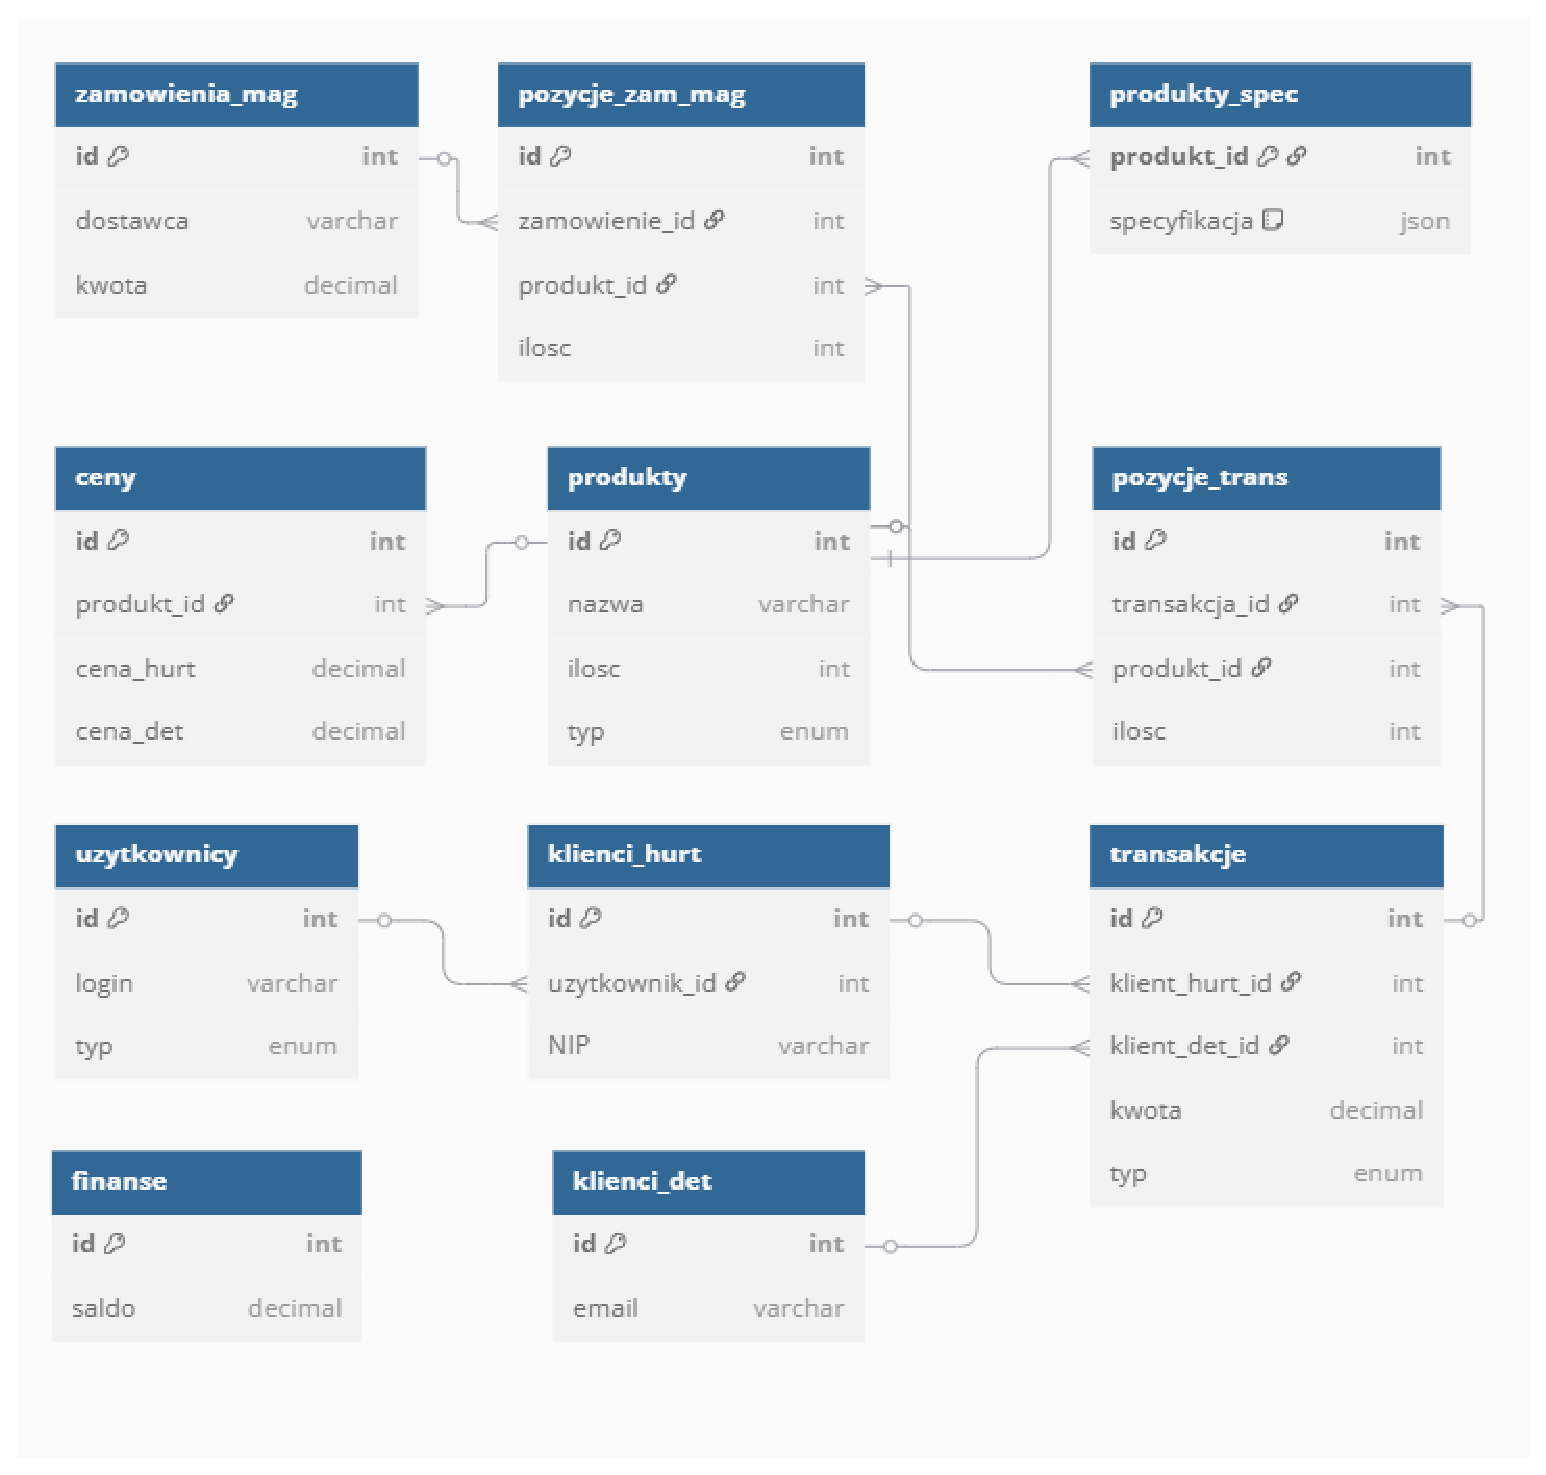
\includegraphics[width=\linewidth]{figures/fig_0001.eps}
    \caption{Schemat bazy danych (ERD) aplikacji sklepu.}
    \label{fig:erd_diagram}
    \small{Źródło: Wygenerowano za pomocą https://dbdiagram.io/}
\end{figure}
\clearpage

\section{Wymagania systemowe}
Uruchomienie projektu w środowisku deweloperskim wymaga zainstalowania i skonfigurowania dwóch głównych narzędzi. Do obsługi bazy danych niezbędny jest pakiet \textbf{XAMPP}, który dostarcza serwer Apache oraz MariaDB (kompatybilny z MySQL). Z kolei do kompilacji i uruchomienia kodu źródłowego aplikacji Java wymagane jest środowisko programistyczne \textbf{IntelliJ IDEA}. Aktualne wymagania systemowe dla obu programów dostępne są na ich oficjalnych stronach:
\begin{itemize}
    \item \textbf{XAMPP:} \url{https://www.apachefriends.org/download.html}
    \item \textbf{IntelliJ IDEA:} \url{https://www.jetbrains.com/help/idea/installation-guide.html#requirements}
\end{itemize}
